% Decision Coprocessor — research compendium paper (LaTeX version).
% Build: pdflatex main.tex && pdflatex main.tex
% Figures: run `make figures` first (they are generated as PDF into figures/).
\documentclass[11pt,a4paper]{article}

\usepackage[T1]{fontenc}
\usepackage[utf8]{inputenc}
\usepackage[margin=2.4cm]{geometry}
\usepackage{amsmath,amssymb}
\usepackage{graphicx}
\usepackage{booktabs}
\usepackage{xcolor}
\usepackage{caption}
\usepackage[hidelinks]{hyperref}
\usepackage{enumitem}

\captionsetup{font=small,labelfont=bf}
\setlist{nosep,leftmargin=1.4em}

\newcommand{\code}[1]{\texttt{#1}}
\newcommand{\dpt}{\ensuremath{\Delta}}

\title{\vspace{-1.2cm}\textbf{Decision Coprocessor: From a Latent Recurrent Sidecar to a Supervised Transition Executor}\\[0.35em]
\large or When Explicit Decomposition Loses to a Fairly Adapted Direct Path}
\author{C. Garrot and the agent mesh (@ag-1\ldots@ag-5)\\
\small Research compendium, snapshot 2026-09-25 --- V1/V2 closed, V2.1 published, V2.2 in progress}
\date{}

\begin{document}
\maketitle

\begin{abstract}
\noindent
Can a small, explicitly computational module improve multi-step decisions made by a small language model without generating intermediate text, on a single 8\,GB consumer GPU? We report a two-part empirical study. \textbf{V1} attached a latent recurrent \emph{sidecar} (2.11\,M parameters) to a frozen Qwen3-0.6B backbone and evaluated it on 53{,}500 oracle-generated problems with a reserved test opened once after pre-registration. The sidecar did not improve depth decisions: $\dpt(\mathrm{R4}-\mathrm{B2}) = -0.59$\,pt $[-1.25;+0.07]$; non-recurrent and unshared-stack controls matched it; recurrence saturated at $k=1$; the latent memory was barely read. An external audit established that the targeted mechanism had never been demonstrated in that assembly: the correction head had direct access to the query and candidate representations, and a final cross-entropy imposed no state progression. \textbf{V2} rebuilt the idea as a \emph{supervised transition executor} on an explicit graph state (92{,}802 parameters, CPU stage): one shared transition, exact state traces as supervision, and an anti-shortcut readout. Stage S established a learned, composed, causally verified transition (trajectory 1.000 on all gates; zero-shot depths 6/8/10/16 at 1.000; stress 399/399; causal $k$-sweep 0.188$\to$1.000). Stage T reconnected language with a LoRA-adapted reader. Under a fairness rule requiring identical adaptation for both paths, the direct text$\to$answer path reached 1.000 dev (causal profile 0.996/0.996/0.988) while the text$\to$graph$\to$executor pipeline plateaued at 0.762 --- $\dpt=-23.84$\,pts $[-28.33;-19.60]$ --- an experience stop for decomposition \emph{on that protocol}. A post-closure validation on eight fresh frozen-checkpoint benches then found a \textbf{depth reversal}: the direct path collapses beyond depth 6 (0.28 at depth 8) while the pipeline holds (0.60), with 123--172/400 complementary items. Pre-registered interface ablations localised the pipeline's bottleneck to \textbf{discretisation}: propagating successor \emph{distributions} from the frozen reader, at zero training cost, restores a depth-invariant accuracy of 0.83--0.86 (depth 1$\to$10), $+25.5$\,pts over discretisation at depth 8 and $+57.25$\,pts over the direct path, with confidence intervals excluding zero on all eight benches. A distributionally retrained reader is running as this snapshot is written. We document the entire evidence chain --- pre-registration, independent QA recomputation, sealed sets, incidents and reserves --- and distil thirteen transferable lessons.
\end{abstract}

\section{Introduction}

Reasoning with small language models on modest hardware invites a specific temptation: making a \emph{small} amount of extra computation look like \emph{deliberation}. Our project began with that hypothesis and ended up producing something more interesting than a confirmation. It asks two questions:

\begin{itemize}
\item \textbf{V1:} Does a small recurrent module appended after the encoding of a frozen backbone improve decisions requiring several dependent operations, at an acceptable real cost on an RTX 3070 Laptop (8\,GB)?
\item \textbf{V2:} Is a transition \emph{learned}, \emph{composed}, and \emph{causally useful} --- \emph{before} reconnecting language?
\end{itemize}

V1 answered with a documented negative. A critical external audit then showed that the negative did not test the intended mechanism: the correction head received the query $q$ and the contextualised candidate $c_i$ directly, so the network could answer without executing any latent composition, and a single final cross-entropy imposed no state progression --- which explains the observed saturation at $k=1$. V2 rebuilt the mechanism in its purest form: a \emph{transition executor} on an explicit graph, supervised by exact intermediate states, with an explicit anti-shortcut readout --- first on structured input (stage S, CPU only), then on text (stage T).

The results form a chain in which every claim is scoped and falsifiable:

\begin{enumerate}
\item \textbf{S demonstrated.} The transition is learned, composed zero-shot to unseen depths, causally useful, robust.
\item \textbf{T refuted under fairness.} With identical LoRA adaptation on both sides, the decomposed pipeline is clearly dominated on short chains ($-23.8$\,pts).
\item \textbf{The refutation is depth-scoped (V2.1).} On fresh frozen-checkpoint benches, the direct path collapses beyond depth 6 while the pipeline holds: $+14$ to $+32$\,pts at depths 6/8/10.
\item \textbf{The remaining gap is the interface (V2.2).} Propagating successor distributions instead of per-edge argmax, at zero training, removes the depth decay (0.83--0.86 invariant), up to $+57$\,pts over the direct path in depth --- leaving $\approx 9$--$12$\,pts to the deterministic ceiling.
\end{enumerate}

\paragraph{Contributions.} A complete reproducible negative on latent recurrent coprocessors over frozen backbones with matched controls and a mechanistic diagnosis (\S\ref{sec:v1}); a supervised transition executor proving learnable, composable, causal depth generalisation with a 93\,K-parameter CPU model (\S\ref{sec:s}); a fairness study showing the apparent benefit of text decomposition ($+5.1$\,pts) becoming a decisive deficit ($-23.8$\,pts) once representation budgets are equalised, with the deficit depth-scoped (\S\ref{sec:t}--\ref{sec:v21}); a zero-training interface repair restoring depth invariance of a frozen reader with CIs excluding zero on 8/8 benches (\S\ref{sec:v22}); and a methodology whose rules measurably changed the conclusions (\S\ref{sec:method}).

\section{Related work and positioning}

Our starting point was the family of \textbf{latent-computation} approaches: Perceiver-style cross-attention to a small latent space~\cite{perceiver}; differentiable cache augmentation of a frozen LLM~\cite{deliberation}; soft chain-of-thought through a fixed assistant~\cite{softcot}; continuous latent reasoning~\cite{coconut}; recurrent refinement of proposed latents for frozen LLMs~\cite{lrt}; continuous latent test-time scaling in other modalities~\cite{listen}. V1's sidecar is architecturally close to this family; its negative result is, in our reading, explained by the \emph{supervision and shortcut structure} rather than by the family.

Control of computation over depth relates to PonderNet~\cite{pondernet} and tiny recursive networks on structured tasks~\cite{tinyrec}. We adopted a fixed budget with an absorbing terminal instead of a learned halting policy, and deferred gating until mechanism utility was demonstrated. Procedural supervision resembles process supervision/distillation~\cite{system2} in spirit, but no natural-language rationale is generated at any point. Our tasks are synthetic and oracle-generated; the closest public benchmark is ProofWriter~\cite{proofwriter}, deliberately not run: our goal was controlled difficulty axes rather than natural-language transfer. Calibration methodology follows~\cite{calibration}, and we publish NLL, Brier and ECE jointly. We claim no new architecture: the contribution is an unusually complete evidence chain for a small-scale question, and two findings we did not expect --- representation fairness can invert an architectural conclusion, and a frozen reader's depth decay can be a discretisation artefact repairable without retraining.

\section{Method}
\label{sec:method}

\paragraph{Verdict frames.} Every claim is published at one of three levels: \emph{experience stop}, \emph{local scientific conclusion}, \emph{product validation} (never claimed). Hypotheses, stop rules and thresholds were written and hashed before runs.

\paragraph{Data.} All data is programmatically generated with exact oracles; every example has a public view (what the model sees) and a private view (answer, trace, depth, group id). Grouping is assigned before variations; variants never cross splits. V1 generated 53{,}500 examples across four families (Horn-rule deduction with established/refuted/undetermined semantics; relational chains; bounded programs; simple controls) with train/dev/router/calibration and three reserved tests (IID, depth 6/8/10, composition). V2's structured family is a relational task: disjoint chains, unique successor, $\ge 3$ terminals, unreachable distractors, opaque renamed entities, shuffled facts. V2's text view is a deterministic French rendering validated against a trivial lexical probe.

\paragraph{Evaluation discipline.} (i) \emph{Pre-registration}: protocol document, hashed config, registry entry before start; scripts committed before use. (ii) \emph{Independent QA}: a separate agent reimplements oracles and recomputes metrics from archived per-item predictions. (iii) \emph{Seals}: V1's reserved test opened once; \code{E5\_eval} and \code{E5v2\_eval} sealed forever with zero artefacts; V2.1 benches evaluation-only; seed 2213 selection-only. (iv) \emph{Statistics}: paired comparisons by group id, coupled grouped bootstrap (2000), 95\,\% CIs, one primary comparison per study, all denominators published. (v) \emph{Mechanism}: full-trajectory accuracy, transition accuracy conditional on a correct state, autonomous roll-out at unseen depths, and paired causal interventions --- probes alone never suffice.

\paragraph{Fairness rules.} \textbf{F1}: any representation advantage must be given identically to the decomposed path and the direct control. \textbf{F2}: adaptation invalidates cached hidden states. \textbf{F3}: no selection on evaluation data. \textbf{F4}: abstention rules pre-registered and symmetric; primary metric all-in, coverage/risk separate.

\section{V1: frozen backbone + latent recurrent sidecar}
\label{sec:v1}

\paragraph{Model.} A frozen \code{Qwen/Qwen3-0.6B} (596\,M parameters, revision pinned) encodes the serialised problem once per example: $H \in \mathbb{R}^{B\times L\times 1024}$. A shared direct head scores each candidate from $q$ (last valid token) and $c_i$ (masked mean of candidate tokens) with features $[q, c_i, q\odot c_i, |q-c_i|]$ (1{,}054{,}209 parameters; baseline \textbf{B2}). A latent sidecar (2{,}110{,}465 trainable parameters) keeps 8 slots of width 256, projects $H$ into keys/values once, applies one \emph{shared} block (cross-attention to memory, self-attention, FFN; residual scale 0.1) $k$ times, then a residual correction $\Delta_i = \mathrm{CorrectionHead}([q, c_i, r_i])$. Budget 0 returns the direct logits exactly. Controls: \textbf{B3} non-recurrent single widened pass (same parameter budget), \textbf{B4} four unshared blocks (comparable cost), \textbf{B1} frozen features, \textbf{B0} priors, \textbf{G4} a gate over $\{0,4\}$ steps.

\begin{figure}[t]
\centering
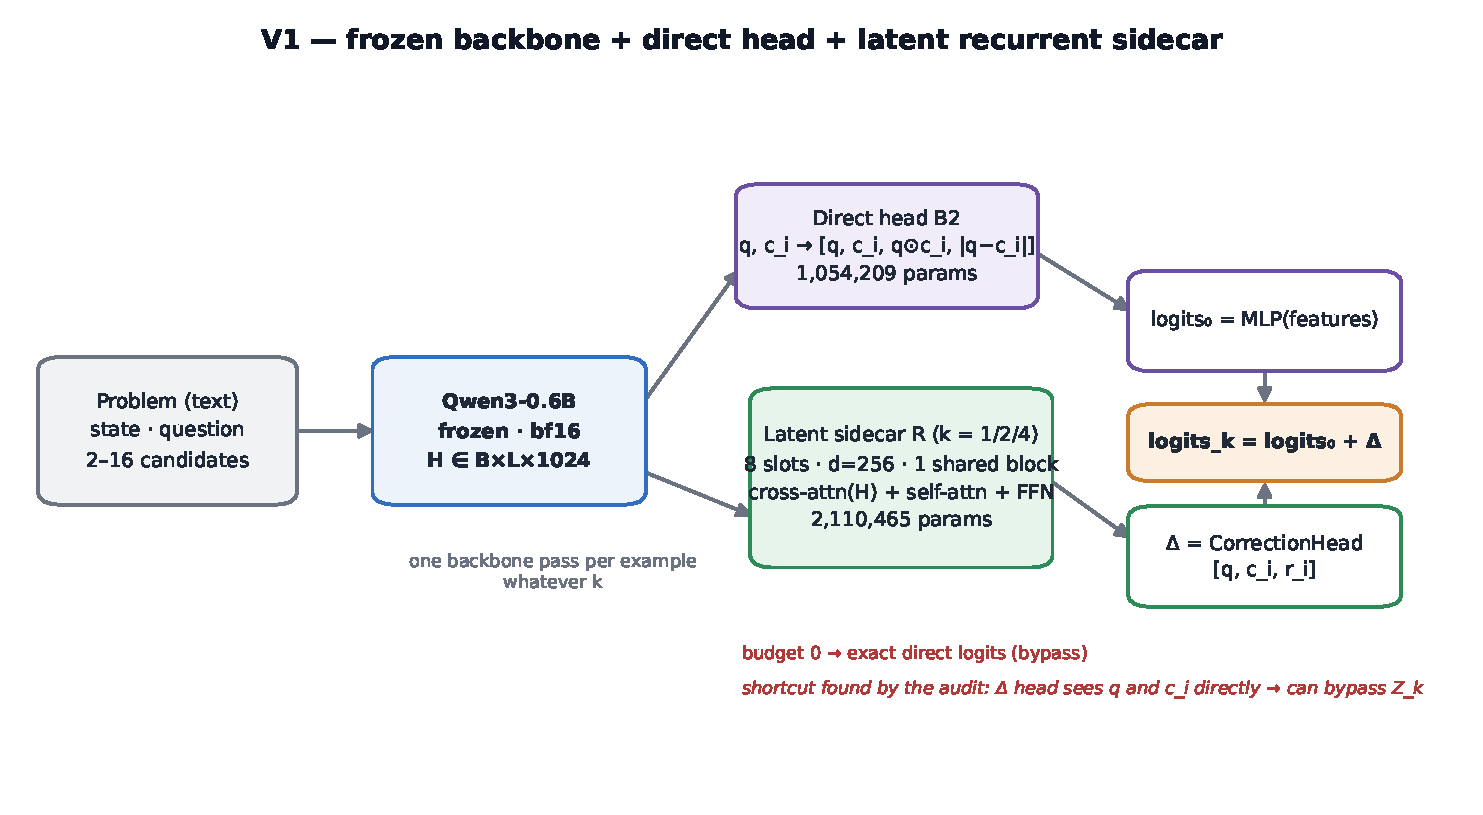
\includegraphics[width=\linewidth]{figures/fig01-v1-architecture.pdf}
\caption{V1 architecture. The sidecar's correction head receives $q$ and $c_i$ directly --- the architectural shortcut identified by the external audit.}
\label{fig:v1arch}
\end{figure}

\paragraph{Protocol.} Phases A (B2, 3 seeds), B (sidecar, 3 seeds, initialised from the matching B2 checkpoint, direct head frozen), C (controls, 3 seeds). AdamW, lr $3\times10^{-4}$, effective batch 32, 1{,}200-step cap ($\approx 1.28$ epoch actually used), bf16 backbone with FP32 trainable modules. Selection on dev; reserved test opened once after pre-registration v2.1; $>512$-token exclusions frozen id-by-id; first latency pass invalidated (laptop clocks) and rerun warm.

\paragraph{Results.} Table~\ref{tab:v1} summarises the reserved test (macro A/B/C over three seeds). The direct head learns clearly; neither the sidecar nor any control improves depth decisions.

\begin{table}[t]
\centering
\caption{V1 reserved test, mean of 3 seeds. $\dpt$ depth is paired vs B2, CI95.}
\label{tab:v1}
\small
\begin{tabular}{lrrrrr}
\toprule
Variant & Params & IID & Depth & Compo. & $\dpt$ depth vs B2 \\
\midrule
\textbf{B2} direct & 1{,}054{,}209 & 0.4884 & \textbf{0.3418} & 0.4081 & --- \\
B3 non-recurrent & 2{,}178{,}177 & 0.4918 & 0.3343 & 0.4070 & $-0.75$ $[-1.40;-0.08]$ \\
B4 unshared $\times4$ & 5{,}270{,}785 & 0.4930 & 0.3382 & 0.4062 & $-0.36$ $[-1.02;+0.32]$ \\
R4 sidecar & 2{,}110{,}465 & 0.4908 & 0.3359 & 0.4073 & $-0.59$ $[-1.25;+0.07]$ \\
G4 gate & 35{,}116 & 0.4934 & 0.3420 & 0.4070 & $-0.62$ (ns) \\
B0 majority & 0 & 0.2785 & 0.3334 & 0.2830 & --- \\
B1 frozen & 0 & 0.2741 & 0.2827 & 0.2715 & --- \\
\bottomrule
\end{tabular}
\end{table}

Further facts: R4 produced 181 corrections against 238 degradations on depth; NLL marginally worse than B2; latency 46.18\,ms (B2) vs 50.04\,ms (R4) at L512 batch 1; VRAM peak 1.199\,GiB; the depth test lost 920/4{,}000 examples to the 512-token limit (81\,\% of family-B depth-10).

\paragraph{Diagnosis and audit.} Diagnostics showed (i) masking or shuffling the memory changed nothing (0 flips/500; $\dpt$logits $\le 0.004$); (ii) steps 2--4 amplified a frozen correction; (iii) information was readable through candidate representations, not the latent state; (iv) per-instance predictions were unstable under option permutation ($\approx 39\%$), shared with the direct head. The external audit added the decisive point: the mechanism could be bypassed and was never forced to progress. \emph{V1 tested an assembly that could avoid reasoning; it did not refute the coprocessor idea.}

\begin{figure}[t]
\centering
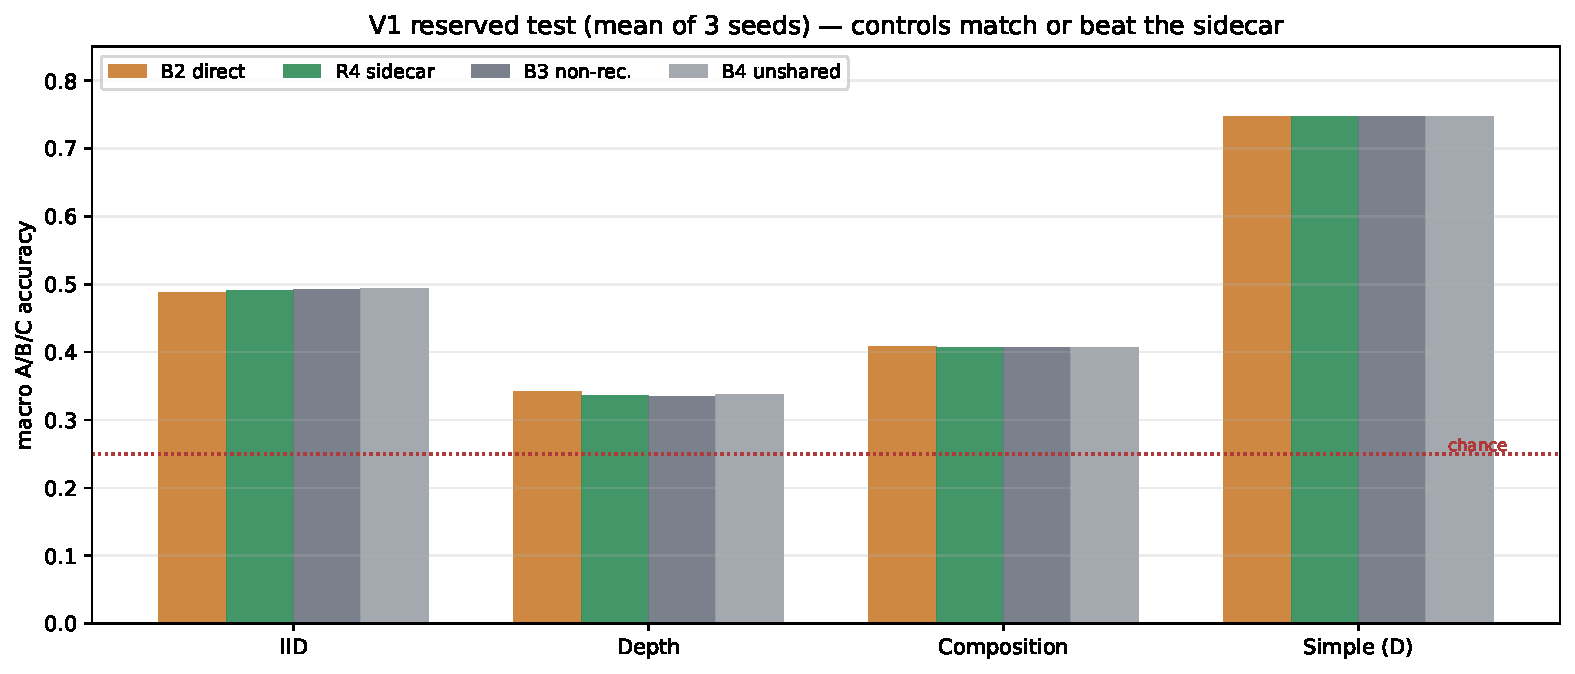
\includegraphics[width=\linewidth]{figures/fig05-v1-main.pdf}
\caption{V1 reserved-test accuracies by split. Controls match or beat the sidecar everywhere.}
\label{fig:v1main}
\end{figure}

\section{V2 stage S: supervised transition executor}
\label{sec:s}

Stage S removes language. A problem is a graph: nodes, directed edges, a start, candidates. The model maintains $s_t=(h_t,p_t)$ --- per-entity vectors and a pointer distribution. Each step:
\begin{align*}
m_i(t) &= \frac{\sum_j p_j\,\phi(h_j,h_i,rel_{ji})}{\sum_j p_j}, &
h_i(t{+}1) &= \mathrm{GRUCell}([m_i,q,p_i],h_i), &
p_t &= \mathrm{softmax}(\mathrm{pointer\_head}(h_t)).
\end{align*}
The final readout scores candidates from the state summary and \emph{raw} candidate features only; the question and contextualised candidates are excluded --- the explicit anti-shortcut correction of the V1 defect. The loss is
\begin{equation}
\mathcal{L} = \mathrm{CE}(\text{answer}) + \alpha \sum_t w_t\,\mathrm{CE}(\text{state}_t,\text{state}^\star_t), \qquad \alpha = 0.5,
\end{equation}
with exact oracle trace targets and weights summing to one (absorbing-terminal mass spread evenly). Budget 16 fixed; $p_0$ is the one-hot start (task constraint, never a free summary); 92{,}802 parameters, CPU only.

\begin{figure}[t]
\centering
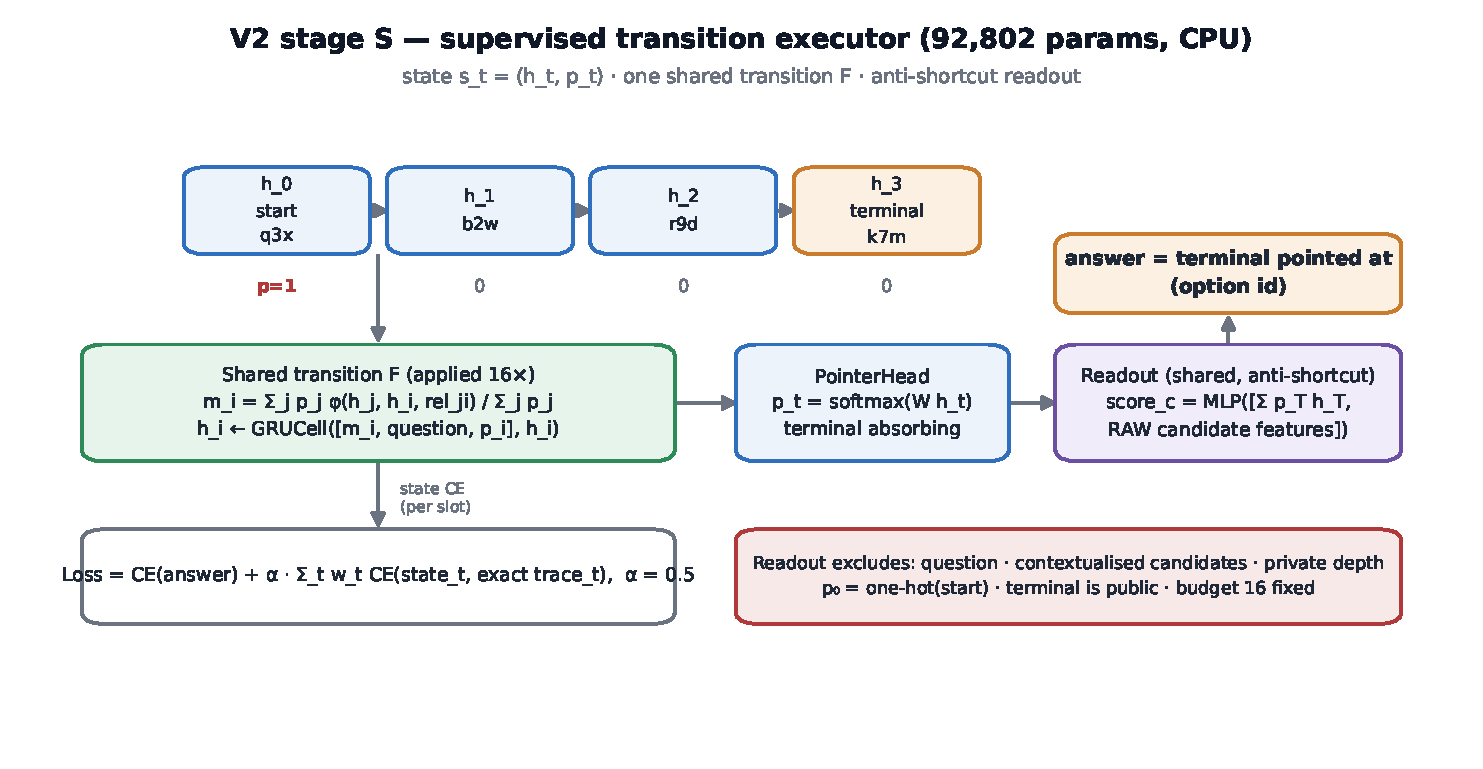
\includegraphics[width=\linewidth]{figures/fig02-v2-executor.pdf}
\caption{The transition executor: shared transition $F$, pointer wavefront, absorbing terminal, anti-shortcut readout.}
\label{fig:v2exec}
\end{figure}

\begin{table}[t]
\centering
\caption{V2 stage-S gates (all CPU).}
\label{tab:s}
\small
\begin{tabular}{lll}
\toprule
Gate & Setting & Result \\
\midrule
E1 & overfit 128 short problems & trajectory \textbf{1.000} (128/128); final 1.000; 452\,s \\
E2 & zero-shot 335 unseen graphs, depth 1--4 & \textbf{919/919 = 1.000}; base 767/767; decisive 152/152 \\
E3 & depths 2/3/4, 13--16 nodes & trajectory \textbf{1.000}; conditional \textbf{1.000}; vs direct 1.000 vs 0.204 \\
E4/E4b & zero-shot 6/8/10/16, 20-node stress & \textbf{399/399 = 1.000}; 0 state divergences; stress 30/30 \\
\bottomrule
\end{tabular}
\end{table}

Two E0 defects had to be fixed first: the pointer was not reinjected ($\approx$2-hop ceiling) and terminals were frozen at initialisation (unreachable ends), both caught by a diagnostic overfit plateau. E3 needed a second attempt: lr $3\times10^{-3}$ collapsed on the full pool (trajectory 0.000) while single-problem, subset and full-pool-at-$10^{-3}$ diagnostics all reached 100\,\% --- an optimisation failure, not an expressivity one. Table~\ref{tab:ksweep} shows the causal $k$-sweep: iterations are necessary and sufficient, and the saturated result at 1.000 holds for depths never trained on (up to 16).

\begin{table}[t]
\centering
\caption{Causal $k$-sweep on one trained checkpoint (same weights).}
\label{tab:ksweep}
\small
\begin{tabular}{lrrrrrr}
\toprule
$k$ & 0 & 1 & 2 & 4 & 8 & 16 \\
\midrule
E3 final answer & 0.188 & 0.271 & 0.522 & \textbf{1.000} & 1.000 & 1.000 \\
E4b final answer & 0.286 & --- & --- & --- & 0.960\,($k{=}10$) & \textbf{1.000} \\
\bottomrule
\end{tabular}
\end{table}

\section{V2 stage T: reconnecting language}
\label{sec:t}

A reader maps French text to the structured memory: a BIO-style mention tagger, fact-level subject/object heads, a question-conditioned start head plus a deterministic containment fallback, and terminals derived from END facts. The pipeline is reader $\to$ exact solver or learned executor (cells (b)/(c)/(cn)); the direct path is an equal-rights text$\to$answer classifier (cell (d)).

\paragraph{Benchmark validation saved the study twice.} E5 v1 looked valid but a trivial lexical probe plus causal interventions exposed a template shortcut: the direct path scored 0.7775 by exploiting a distributional template lever. The bench was archived as defective, its sealed eval remained closed forever, and E5v2 was rebuilt (shuffled decks, per-option wrappers, recall formulations, distractor-length post-pass). On E5v2 the lexical probe is at chance (0.218--0.243 vs 0.221) and the direct path drops to 0.326. Frozen-reader iterations improved edges from 0.397 to 0.725 and fixed the start, but plateaued at solve 0.248 over three bounded iterations; a controlled-noise experiment showed the apparent executor advantage over the exact solver was an abstention-policy artefact, not robustness. The verdict was a documented local failure with the benefit published as a grey zone.

\paragraph{Representation fairness inverts the conclusion.} The final V2 experiment gave \emph{both} paths the same LoRA adaptation (r16/$\alpha$32 on q/k/v/o, dropout 0.05, two learning rates, 1200 steps, seed 17, caches invalidated). The reader passed all four gates for the first time (entities 1.000, edges 0.9278, start 1.000, solve 0.7616; validity 0.917), validating the pre-registered hypothesis that adaptation --- not head architecture --- was the extraction bottleneck. But the same adaptation lifted the direct path to 1.000: $\dpt(c-d) = -23.84$\,pts $[-28.33;-19.60]$, with the direct path causally composing (0.996/0.996/0.988). The contrast is the central result:

\begin{table}[t]
\centering
\caption{The fairness reversal (dev, n=411).}
\label{tab:reversal}
\small
\begin{tabular}{lrrrl}
\toprule
Regime & Pipeline (c) & Direct (d) & $\dpt(c-d)$ & Reading \\
\midrule
Frozen backbone & 0.338 & 0.287 & $+5.1$ $[-1.7;+11.7]$ & grey zone --- crippled baseline \\
Adapted (fair) & 0.762 & \textbf{1.000} & $-23.84$ $[-28.33;-19.60]$ & decomposition dominated \\
\bottomrule
\end{tabular}
\end{table}

\begin{figure}[t]
\centering
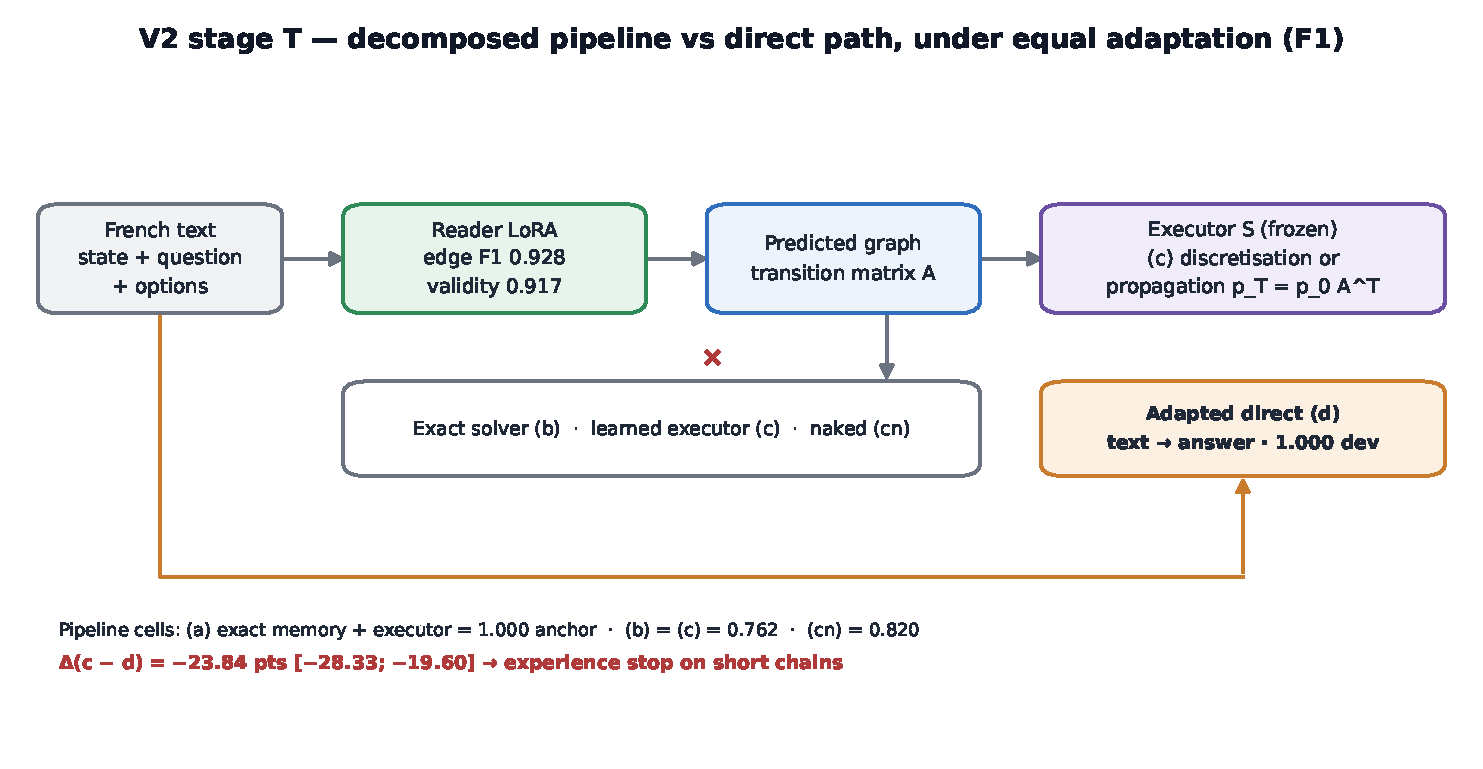
\includegraphics[width=\linewidth]{figures/fig03-v2-pipeline.pdf}
\caption{Stage T: the decomposed pipeline and the equal-rights direct path.}
\label{fig:pipeline}
\end{figure}

\section{V2.1: frozen-checkpoint validation and the depth reversal}
\label{sec:v21}

No retraining; frozen artefacts; eight fresh benches of 400 items (seeds 2205--2212): short depth 1--4, depths 6/8/10, surface paraphrases, extra distractors, permuted options, changed start; $K\in\{4,5,6\}$, $\le 20$ nodes, French; strict signature disjunction; thresholds frozen before any prediction. Oracle diagnostics were published in separate tables and never counted as scores.

\begin{table}[t]
\centering
\caption{V2.1 results (n=400 per bench, frozen checkpoints).}
\label{tab:v21}
\small
\begin{tabular}{lrrrr}
\toprule
Bench & (a) anchor & (c) pipeline & (d) direct & $\dpt(c-d)$ [CI95] \\
\midrule
B1 short (1--4) & 1.000 & 0.800 & 0.9375 & $-13.75$ \\
B5 surface & 1.000 & 0.810 & 0.940 & $-13.00$ \\
B6 distractors & 1.000 & 0.772 & 0.9375 & $-16.50$ \\
B7 options & 1.000 & 0.800 & 0.940 & $-14.00$ \\
B8 other start & 1.000 & 0.765 & 0.840 & $-7.50$ \\
\textbf{B2 depth 6} & 1.000 & 0.667 & 0.525 & $\mathbf{+14.25}$ $[+7.5;+21.0]$ \\
\textbf{B3 depth 8} & 1.000 & 0.598 & 0.280 & $\mathbf{+31.75}$ $[+25.0;+38.5]$ \\
\textbf{B4 depth 10} & 1.000 & 0.560 & 0.3075 & $\mathbf{+25.25}$ $[+18.3;+32.0]$ \\
\bottomrule
\end{tabular}
\end{table}

\begin{figure}[t]
\centering
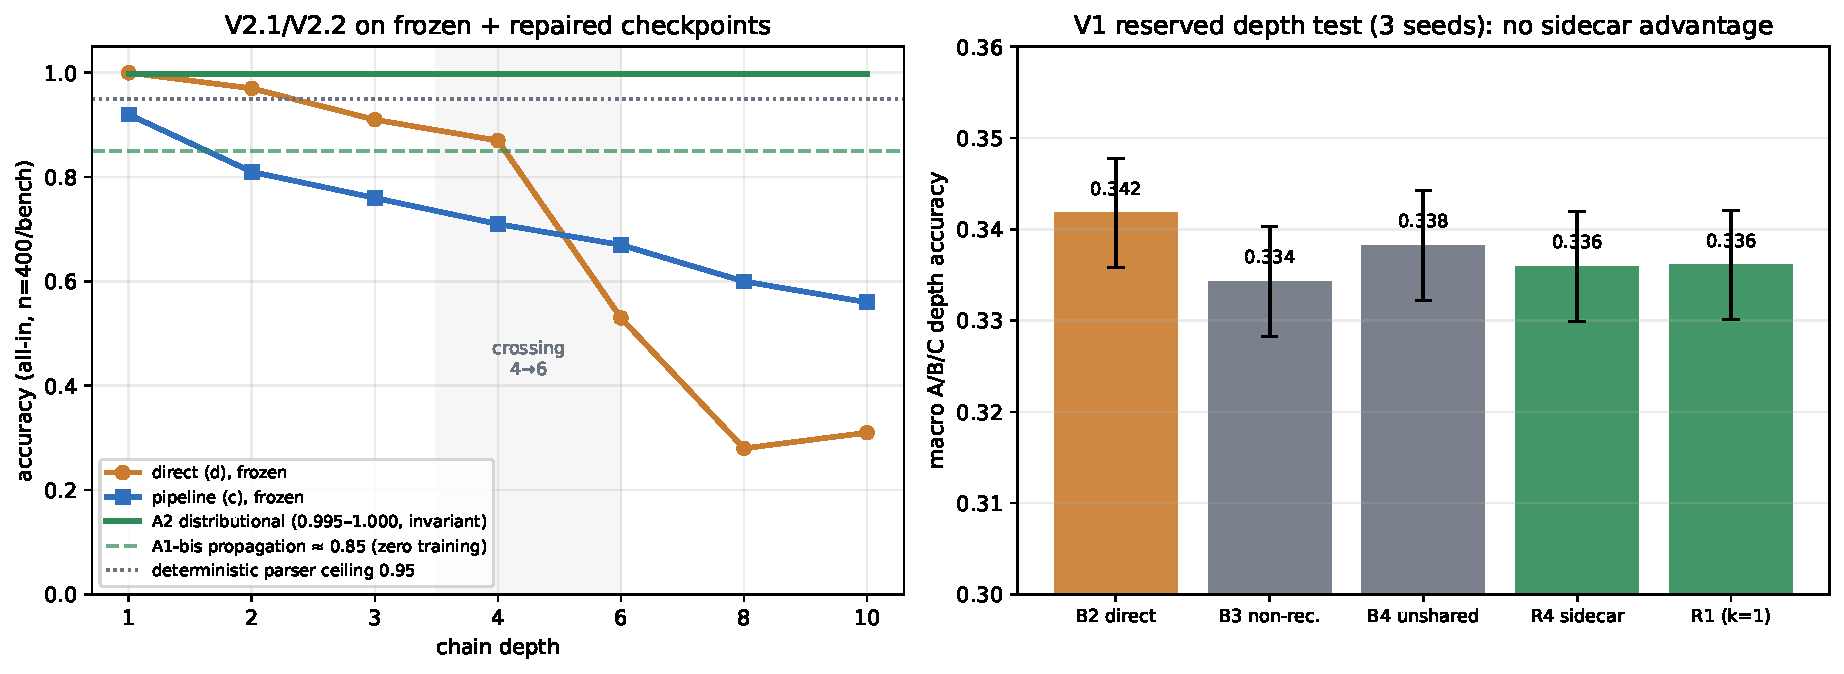
\includegraphics[width=\linewidth]{figures/fig04-depth-curves.pdf}
\caption{Left: the depth reversal --- accuracy vs depth on frozen checkpoints, with the A1-bis propagation level. Right: V1 depth accuracy by variant (no sidecar advantage).}
\label{fig:depth}
\end{figure}

\paragraph{Localisation.} (a) $=1.000$ everywhere, including depth 10: the executor composes; the deficit is entirely in reading. A path-only oracle corrector recovers 0.950/0.965/0.9825/0.9825 (B1--B4) vs baseline 0.800/0.667/0.598/0.560: \emph{only the useful-path edges matter}. Complementarity reaches 123/172/163 of 400 items at depths 6/8/10 while the direct path's NLL grows 0.59$\to$8.85 nats --- a routing signal to exploit, after measuring the oracle router bound. A deterministic parser bounded to the templates achieves coverage 1.0000 and agreement 1.0000 on 3{,}200/3{,}200 items: the information is in the public text; the deficit is in learned extraction and the interface. Numbers are environment-labelled (CPU vs GPU can differ by $\approx6$\,pts on this near-tie reader).

\section{V2.2: interface ablations (ongoing)}
\label{sec:v22}

\textbf{Hypothesis (pre-registered):} the depth deficit comes from discretisation at the interface --- per-edge argmax kills a chain on a single missing edge --- not from the reader's information (edge F1 0.93; parser ceiling 0.95). Propagating distributions $p_{t+1}=p_tA$ should recover a measurable part of the gap.

\paragraph{A1: failure with a real cause.} A1 propagated distributions from the frozen reader using the \emph{bilinear} successor head, which is never supervised in fact mode (top-1 0.054 $\approx$ chance): it propagated noise (c\_prop 0.19--0.32 vs discretisation 0.56--0.81, $\dpt=-38.25$\,pts). The failure is documented; the initial mass-leak explanation was withdrawn.

\paragraph{A1-bis: zero-training repair (PASS).} The transition matrix is built from the supervised fact-level heads:
\begin{equation}
A[u,v] = \sum_f P(\text{subject}_f=u)\,P(\text{object}_f=v),
\end{equation}
with terminal self-loop, absorbing UNKNOWN sink for missing subject mass, no silent renormalisation, stable tie-break. No training, frozen checkpoints, sealed benches.

\begin{table}[t]
\centering
\caption{A1-bis (zero training): distribution propagation vs discretisation and vs the adapted direct path.}
\label{tab:a1bis}
\small
\begin{tabular}{lrrrr}
\toprule
Bench & c\_prop & c\_discret & $\dpt$ vs discret [CI95] & $\dpt$ vs direct \\
\midrule
B1 short & 0.8550 & 0.8000 & $+5.50$ $[+1.50;+9.25]$ & $-8.25$ \\
B2 depth 6 & 0.8375 & 0.6675 & $+17.00$ $[+12.50;+21.50]$ & $+31.25$ \\
\textbf{B3 depth 8} & 0.8525 & 0.5975 & $\mathbf{+25.50}$ $[+20.75;+30.00]$ & $\mathbf{+57.25}$ \\
B4 depth 10 & 0.8550 & 0.5600 & $+29.50$ $[+24.50;+34.75]$ & $+54.75$ \\
B5 surface & 0.8525 & 0.8100 & $+4.25$ $[+0.25;+8.25]$ & $-8.75$ \\
B6 distractors & 0.8325 & 0.7725 & $+6.00$ $[+2.25;+9.75]$ & $-10.50$ \\
B7 options & 0.8550 & 0.8000 & $+5.50$ $[+1.50;+9.25]$ & $-8.50$ \\
B8 other start & 0.8575 & 0.7650 & $+9.25$ $[+5.25;+13.50]$ & $+1.75$ \\
\bottomrule
\end{tabular}
\end{table}

\begin{figure}[t]
\centering
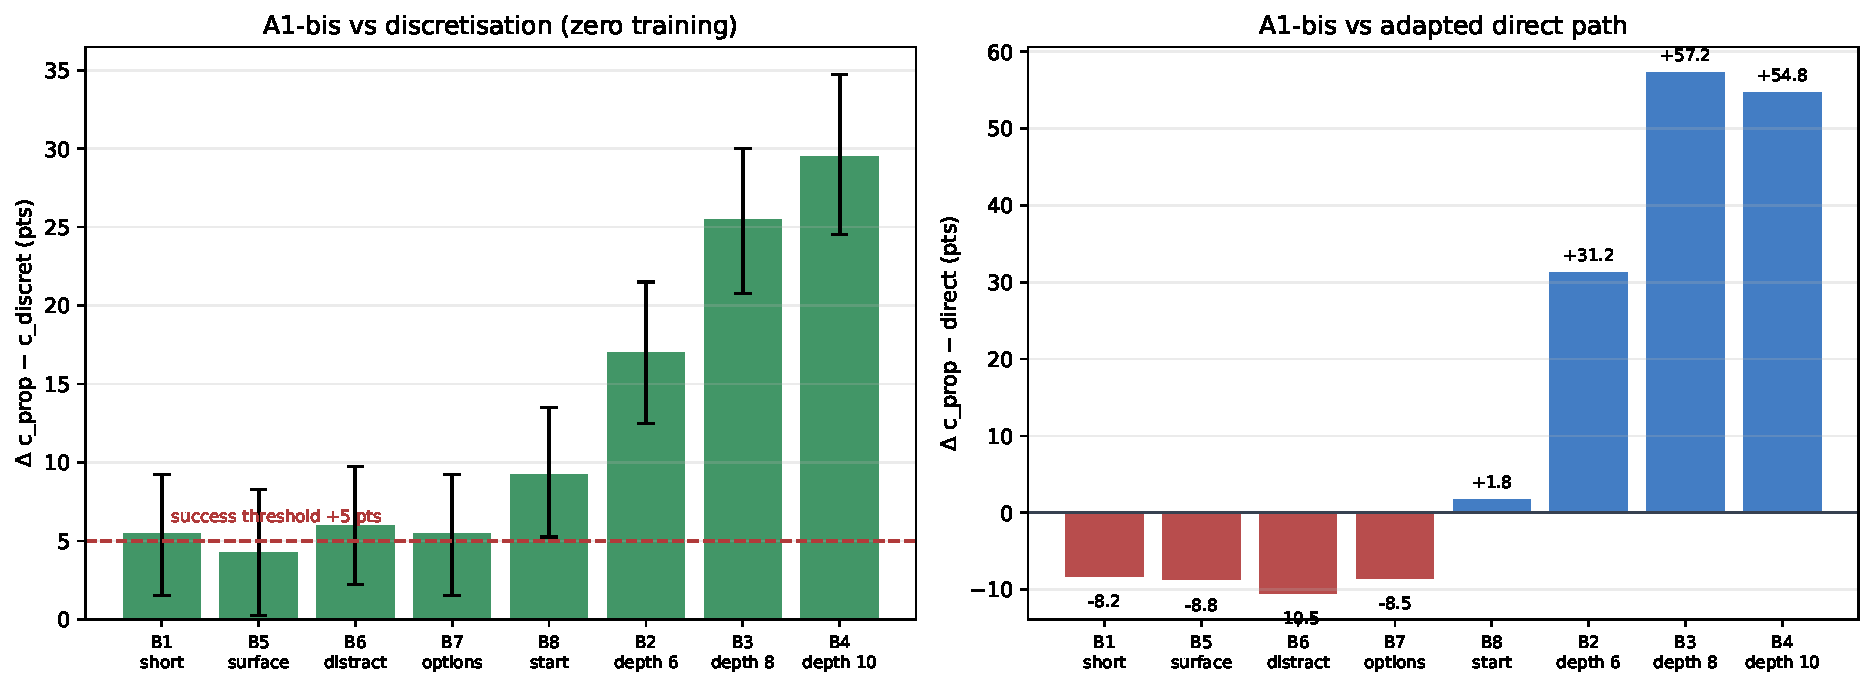
\includegraphics[width=\linewidth]{figures/fig06-a1bis.pdf}
\caption{A1-bis per bench: vs discretisation (left) and vs the adapted direct path (right). CIs exclude zero on 8/8 benches against discretisation.}
\label{fig:a1bis}
\end{figure}

\textbf{c\_prop $\approx$ 0.83--0.86, invariant from depth 1 to depth 10}, versus the discretisation decay 0.80$\to$0.56. All eight CIs exclude zero; the main criterion (B3 $\ge +5$\,pts) is cleared fivefold; short-chain non-regression holds. Remaining gap to the 0.95 template-parser ceiling: $\approx9$--$12$\,pts.

\paragraph{A2 (running at snapshot).} A2 retrains the reader with distributional supervision: transitions trained as distributions, propagation inside the graph so the answer CE reaches edge distributions, per-step state supervision, and an explicit UNKNOWN class (absence of information $\ne$ terminal; absorbing sink). It initialises from the frozen best reader, reuses the identical LoRA recipe, and selects on a fresh bench (seed 2213, selection only). Run 1 was cancelled (inactive gradient checkpointing $\to$ OOM; a gold/predicted mismatch corrupted the selection metric); the run was relaunched with the frozen config unchanged. At snapshot (step 300/1200), selection c\_prop $=0.99$ with discretisation 0.91--0.97. \emph{No conclusion is drawn from a running experiment.}

\section{Discussion}

\paragraph{What the project established.} (1) The mechanism is real when isolated: a tiny supervised executor learns an operator, composes it beyond training depth, and passes causal interventions with zero state divergence. (2) The benchmark can dominate the conclusion: a defective text bench produced a 0.78 ``strong direct baseline''; the corrected bench produced 0.33. (3) Fairness can invert an architectural verdict: $+5.1$\,pts (frozen) $\to$ $-23.8$\,pts (adapted). (4) The direct path is not depth-robust: beyond depth 6 it collapses (0.28 at depth 8) while the pipeline holds (0.60). (5) The pipeline's remaining gap is the interface, partially repairable for free: distribution propagation restores depth invariance of a frozen reader; what remains is a distributional-reader problem that A2 addresses with training.

\paragraph{The pattern.} The two turns mirror each other: V1 failed because the mechanism was optional; V2-T ``failed'' because the comparison was unfair to the baseline. Both times the fix was to remove a shortcut or an asymmetry, not to add capacity. Our most reliable heuristic became: \emph{before interpreting a gap, verify that the losing side was not architecturally prevented from winning, and that the winning side was not exploiting a defect of the benchmark.}

\paragraph{Scope.} Stage S is a local conclusion about a controlled relational task, not about language. Stage T's refutation is depth-scoped. The 1.000 direct number is a single run on dev with selection on the same dev: a \emph{best reference}, not a validated result. V2.2/A2 is running and is not part of the conclusions.

\section{Limitations and threats to validity}

\begin{enumerate}
\item \textbf{Scale:} one 0.6\,B backbone, one 8\,GB GPU, synthetic French tasks; no external benchmark run.
\item \textbf{Seeds and confirmation:} one training seed per path in V2-T/V2.1/V2.2; CIs conditional on measured checkpoints; no confirmatory test opened for T.
\item \textbf{Adaptive campaigns:} dev used for checkpoint selection; best-of-run values are exploratory.
\item \textbf{Data coverage:} V1 depth test lost 23\,\% of examples to the 512-token limit; broken-chain ``det'' structurally absent (0/411).
\item \textbf{Environment sensitivity:} CPU/GPU reader inference differs by $\approx6$\,pts on near ties; later runs use a declared eps tie-break.
\item \textbf{Synthetic-bench ceiling:} the template parser's 0.95 is an existence proof, not a learned-reader target.
\item \textbf{No product claim:} latency, robustness, safety and OOD behaviour are out of scope.
\end{enumerate}

\section{Conclusion}

Stage S shows the mechanism is learnable and verifiable at 93\,K parameters. Stage T shows that, under equal representation budgets, explicit decomposition loses to a direct path on short chains --- while a fresh frozen-checkpoint validation shows the direct path itself collapsing with depth, and a zero-training interface repair makes the decomposed reader depth-invariant. The through-line is methodological: hashed pre-registration, independent recomputation, sealed sets, paired causal interventions, mechanism-before-benefit precedence, and a representation-fairness rule that twice forced us to withdraw a conclusion we had reason to like. The project's negative results are, we believe, its most durable output: they are cheap to obtain on consumer hardware and unusually specific about \emph{why} the ideas they reject did not work here.

\appendix

\section{Data contracts (summary)}
Public/private split enforced by tests; V1: 53{,}500 examples across families A--D, group-based splits, three reserved tests, id-by-id 512-token exclusions. V2-S: unique successor, acyclic, $\ge3$ terminals, unreachable distractors, trace weights summing to one. V2-T: deterministic French rendering with 8/6/5/7 formulation decks, recall and second-declaration noise, probe at chance. V2.1: 8 benches $\times$ 400, seeds 2205--2212, strict disjunction. V2.2: selection bench seed 2213 (selection only); UNKNOWN semantics fixed before use.

\section{Gate criteria (summary)}
V2 E0--E2: 42 data-contract tests; E1 $\ge0.99$ (achieved 1.000); E2 $\ge0.98$ (1.000). E3--E4: autonomous $\ge0.90$ (1.000); conditional $\ge0.98$ (1.000); zero-shot depths 6/8/10/16 (1.000). E5: entities $\ge0.85$; edges $\ge0.65$; start $\ge0.50$; solve $\ge0.35$; conclusion grid with mechanism precedence. V2.2: $\dpt(c\_prop-c\_discret) \ge +5.0$\,pts on B3 with lower CI $>0$; B1 non-regression $\ge -2.0$\,pts; eps $=10^{-3}$.

\section{Artefacts and reproduction}
Source repositories: \code{decision-coprocessor/} (20 commits) and \code{decision-coprocessor-v2/} (51 commits at snapshot). Frozen bundles reload-verified (V1: 0.0; V2: 8/8+8/8, 14/14 hashes). Registries: \code{experiment\_registry.jsonl}, \code{costs.jsonl}, \code{research\_register.md} (REG-01\ldots REG-75). Every figure is regenerated by \code{figures/make\_figures.py} from the published numbers.

\begin{thebibliography}{99}
\small
\bibitem{perceiver} A. Jaegle et al. Perceiver: General Perception with Iterative Attention. arXiv:2103.03206, 2021.
\bibitem{deliberation} Deliberation in Latent Space via Differentiable Cache Augmentation. arXiv:2412.17747, 2024.
\bibitem{softcot} SoftCoT: Soft Chain-of-Thought for Efficient Reasoning with LLMs. ACL 2025.
\bibitem{coconut} Training Large Language Models to Reason in a Continuous Latent Space. arXiv:2412.06769, 2024.
\bibitem{lrt} Latent Recurrent Thoughts: Recurrent Refinement of Proposed Latents for Reasoning with Frozen LLMs. arXiv:2609.01117, 2026.
\bibitem{listen} Listen, Think, Transcribe: Continuous Latent Test-Time Scaling for ASR. arXiv:2607.05051, 2026.
\bibitem{pondernet} A. Banino et al. PonderNet: Learning to Ponder. arXiv:2107.05407, 2021.
\bibitem{tinyrec} Less is More: Recursive Reasoning with Tiny Networks. arXiv:2510.04871, 2025.
\bibitem{system2} Distilling System 2 into System 1. arXiv:2407.06023, 2024.
\bibitem{calibration} C. Guo et al. On Calibration of Modern Neural Networks. arXiv:1706.04599, 2017.
\bibitem{proofwriter} O. Tafjord et al. ProofWriter. arXiv:2012.13048, 2020.
\bibitem{qwen} Qwen3-0.6B model card. \url{https://huggingface.co/Qwen/Qwen3-0.6B}
\bibitem{eos} Decision 1.0 Eos 0.8B model card. \url{https://huggingface.co/llm-semantic-router/Decision-1.0-Eos-0.8B}
\bibitem{jev} NanoJev model card. \url{https://huggingface.co/C-Tianyu/NanoJev}
\bibitem{lux} Decision 1.0 Lux 9B --- METHODS.md.
\bibitem{iclr26} Rethinking LLM Reasoning: From Explicit Trajectories to Latent Representations. ICLR 2026.
\end{thebibliography}

\end{document}
